\documentclass[abstract=on,10pt,a4paper,bibliography=totocnumbered]{article}
\usepackage[paper=a4paper,left=35mm,right=35mm,top=25mm,bottom=30mm]{geometry}
\usepackage[doublespacing]{setspace}
\usepackage[english]{babel}
\usepackage[utf8]{inputenc}
\usepackage[round]{natbib}
\usepackage{amsmath}
\usepackage{colortbl}
\usepackage{amsfonts}
\usepackage{amssymb}
\usepackage{gensymb}
\usepackage{graphicx}
\usepackage{tikz}
\usepackage{enumerate}
\usepackage{enumitem}
\usepackage{subcaption}
\usepackage{booktabs}
\usepackage[hidelinks]{hyperref}
\usepackage[nameinlink]{cleveref}
% \usepackage{lineno}
\usepackage{multirow}
\usepackage{arydshln}
\usepackage[flushleft]{threeparttable}
\usepackage[nomarkers, nolists]{endfloat}
\usepackage[colorinlistoftodos]{todonotes}
\usepackage{scalerel}
\usepackage{tikz}
\usetikzlibrary{svg.path}

%------------------------------------------------------------------------------
%	Some Styling
%------------------------------------------------------------------------------
% Creating some TikZ styles
\tikzset{
  nonterminal/.style = {rectangle
    , minimum size = 6mm
    , very thick
    , draw = black!
  }
}

% Changing the style of captions in figures etc.
\captionsetup{labelfont=bf, format=plain, font=small}

% Change how equations are referenced
\renewcommand{\theequation}{Equation \arabic{equation}}%

% To be able to put an ORCID
\definecolor{orcidlogocol}{HTML}{A6CE39}
\tikzset{
  orcidlogo/.pic={
    \fill[orcidlogocol] svg{M256,128c0,70.7-57.3,128-128,128C57.3,256,0,198.7,0,128C0,57.3,57.3,0,128,0C198.7,0,256,57.3,256,128z};
    \fill[white] svg{M86.3,186.2H70.9V79.1h15.4v48.4V186.2z}
                 svg{M108.9,79.1h41.6c39.6,0,57,28.3,57,53.6c0,27.5-21.5,53.6-56.8,53.6h-41.8V79.1z M124.3,172.4h24.5c34.9,0,42.9-26.5,42.9-39.7c0-21.5-13.7-39.7-43.7-39.7h-23.7V172.4z}
                 svg{M88.7,56.8c0,5.5-4.5,10.1-10.1,10.1c-5.6,0-10.1-4.6-10.1-10.1c0-5.6,4.5-10.1,10.1-10.1C84.2,46.7,88.7,51.3,88.7,56.8z};
  }
}
\newcommand\orcid[1]{\href{https://orcid.org/#1}{\mbox{\scalerel*{

\begin{tikzpicture}[yscale=-1,transform shape]
  \pic{orcidlogo};
\end{tikzpicture}
}{|}}}}

%------------------------------------------------------------------------------
%	Titlepage: Header
%------------------------------------------------------------------------------
% \title{Flooding of the Okavango Delta influences Connectivity for Dispersing
% African Wild Dogs}
\title{African Wild Dog Dispersal and Connectivity under Climate Change -
Lessons Learned from Seasonal Flood Extremes}

% List of Authors
\author{
  David D. Hofmann\textsuperscript{1,2,\S} \orcid{0000-0003-3477-4365} \and
  Dominik M. Behr\textsuperscript{1,2} \orcid{0000-0001-7378-8538} \and
  John W. McNutt\textsuperscript{2} \and
  Arpat Ozgul\textsuperscript{1,2} \orcid{0000-0001-7477-2642} \and
  Gabriele Cozzi\textsuperscript{1,2} \orcid{0000-0002-1744-1940}
}

% Reduce spacing between authors
\makeatletter
\def\and{%
  \end{tabular}%
  \hskip -0.5em \@plus.17fil\relax
  \begin{tabular}[t]{c}}
\makeatother

% Current Date
% \date{\today}

% And here the masterpiece begins
\begin{document}

% Change page numbering
\pagenumbering{gobble}

% Required to be able to cite
\bibliographystyle{apalike}

% Create Titlepage
\maketitle

%------------------------------------------------------------------------------
%	Titlepage: Additional Info
%------------------------------------------------------------------------------
\begin{flushleft}

\vspace{0.5cm}

\textsuperscript{1} Department of Evolutionary Biology and Environmental
Studies, University of Zurich, Winterthurerstarsse 190, 8057 Zurich,
Switzerland.

\textsuperscript{2} Botswana Predator Conservation Program, Wild Entrust,
Private Bag 13, Maun, Botswana.

\textsuperscript{\S} Corresponding author: david.hofmann2@uzh.ch

\vspace{4cm}

\textbf{Running Title:} African Wild Dog Dispersal in a Changing Climate:
Lessons Learned from Seasonal Flood Extremes

\vspace{0.5cm}

\textbf{Keywords:} movement, connectivity, climate change, seasonality,
dispersal, conservation, individual-based simulations, step-selection

\end{flushleft}

%------------------------------------------------------------------------------
%	Abstract
%------------------------------------------------------------------------------
\newpage
\begin{abstract}
Climate change is expected to profoundly impact the life history of wild-living
animal populations. While the impacts of climate change on the demographics of
local subpopulations have been studied repeatedly, little is known about the
consequences for dispersal and connectivity.

We capitalize on a ``natural experimental setup'', the flood-pulse driven change
in surface-water across the Okavango Delta in northern Botswana, to investigate
the impact of changing environmental conditions on dispersal patterns and
connectivity of the endangered African wild dog (\textit{Lycaon pictus}). For
this, we simulate dispersal trajectories across the Okavango Delta under two
extreme scenarios that serve to represent environmental conditions akin to those
expected under continued climate change; one assuming a maximum flood, one
assuming a minimum flood.

During maximum flood, the Okavango Delta poses an important dispersal barrier
that reduces dispersal prospects in increases dispersal durations between
distinct areas. Across the entire study area, we observe
$\input{99_NumberReachingOthersPercentage.tex}$\% lower dispersal success and
$\input{99_StepsToReachingOthersPercentage.tex}$\% longer dispersal durations
during maximum flood. Most notably, dispersal into the central habitats of the
Okavango Delta is reduced by $\input{99_NumberReachingArea6Percentage.tex}$\%
with an accompanied increase in dispersal durations of
$\input{99_StepsToReachingArea6Percentage.tex}$\%. Depending on the flood,
dispersal corridors traversed different areas and dispersers moved into
proximity of different human-dominated areas.

Whilst the exact impacts of climate change on the flooding regime of the
Okavango Delta remain unknown, our results suggest that connectivity will vastly
differ depending on future flood conditions. Acknowledging such differences will
be key to design effective conservation strategies, especially in light of
ongoing climate change. Since we highlight critical dispersal corridors and
human-wildlife conflict zones for two distinct future scenarios, our results
will facilitate the evidence-based conservation of the endangered African wild
dog.

\end{abstract}

%------------------------------------------------------------------------------
%	Main Text
%------------------------------------------------------------------------------
\newpage

\onehalfspacing
\tableofcontents
\doublespacing

% Change page numbering
\newpage
\pagenumbering{arabic}

% Create linenumbers
% \linenumbers

\section{Introduction}
\subsection{Climate Change and Dispersal}
Climate change is expected to profoundly impact ecosystems across the globe with
far-reaching consequences for the species living therein \citep{Ozgul.2010,
 Radchuk.2019, IPCC.2022}. By altering environmental conditions, climate change
affects animal behavior \citep{Fuller.2016}, resource availability
\citep{Durant.2007}, population dynamics \citep{Paniw.2021}, and the
distribution of wild living animal populations \citep{Thomas.2004,
 Thuiller.2006}. An important life-history pathway through which species may
mediate the negative consequences of climate change is dispersal
\citep{Anderson.2012}, i.e. the movement of individuals away from their natal
location to the site of first reproduction \citep{Clobert.2012}. Through
dispersal, species may adapt to climate change by tracking favorable habitat
conditions \citep{Raia.2012} and by shifting into a different region of their
fundamental niche \citep{Kokko.2006}. Dispersal also facilitates the
colonization empty habitats \citep{Gustafson.1996, Hanski.1999a,
 MacArthur.2001}, promotes the reinforcement of weakened and small subpopulations
\citep{Brown.1977}, and safeguards genetic diversity \citep{Frankham.2002,
 Leigh.2012, Baguette.2013}, thus providing additional resilience against
changing environmental conditions \citep{Kokko.2006, Fahrig.2003}.

\subsection{Connectivity}
While dispersal offers a means to offset the negative demographic consequences
of climate change \citep{Kokko.2006, Hodgson.2009, Travis.2013}, it itself is a
function of climatic and environmental conditions (e.g. \citealp{Elliot.2014,
 Behr.2020}). The link between dispersal and the environment can either be
indirect, for example if the propensity of individuals to disperse depends on
environmental conditions, or direct, when the biophysical environment through
which dispersers move affects dispersal prospects \citep{Travis.2013}. The
latter highlights that dispersal is also inextricably linked to the concept
landscape connectivity \citep{Baguette.2013}, which is understood as the degree
to which the landscape facilitates or impedes movements \citep{Taylor.1993}. A
sufficient degree of landscape connectivity is thus a critical prerequisite for
successful dispersal \citep{Fahrig.2003}, yet the continued degradation and
destruction habitats worldwide continues to imperil the dispersal prospects of
many species \citep{Melbourne.2008, Sawyer.2011}. Conservation strategies that
aim at facilitating dispersal by improving landscape connectivity are therefore
often viewed as pinnacle of all conservation strategies \citep{Heller.2009}.
Despite this, our understanding of dispersal and its implications for
connectivity is limited, especially in light of changing environmental
conditions.

\subsection{Modeling Connectivity}
To study dispersal and connectivity, various modeling techniques have emerged
(see e.g. \citealp{Etherington.2016} and \citealp{Diniz.2019} for overviews).
Initially, the techniques were limited to examining structural aspects of
connectivity by focusing on the composition and configuration of habitat
patches, while ignoring species' responses to the landscape matrix
\citep{Tischendorf.2000, Doerr.2011}. With the increasing availability of
telemetry data and methods to study species' habitat and movement preferences
\citep{Boyce.2002, Fortin.2009, Cushman.2010, Avgar.2016}, preferably during
dispersal \citep{Elliot.2014}, however, the focus has shifted towards a more
functional view on connectivity, which also takes into account how species
interact with their surroundings \citep{Tischendorf.2000, Doerr.2011}.
Currently, the most prominent \textit{functional} connectivity models are based
on least-cost path analysis (LCPA, \citealp{Adriaensen.2003}) and circuit theory
(CT, \citealp{McRae.2008}), two graph-based methods that estimate conductance of
the landscape by means of a resistance (or inversely permeability) surface
\citep{Zeller.2012}. Such a surface is meant to reflect the ease or willingness
at which the focal species traverses a specific area and is generated by
consolidating multiple habitat layers into a single layer of resistance
\citep{Zeller.2012}. Since both LCPA and CT approaches make assumptions that are
rarely met by dispersing individuals, individual-based movement models (IBMMs),
in which dispersal movements are simulated explicitly, have also gained some
momentum \citep{Kanagaraj.2013, Allen.2016, Hauenstein.2019, Diniz.2019,
 Zeller.2020, UnnithanKumar.2022, UnnithanKumar.2022a, Hofmann.2023}. IBMMs
provide great modeling flexibility and are thus considered powerful tools for
examining connectivity under different landscape configurations
\citep{Littlefield.2019, UnnithanKumar.2022a}. However, most connectivity
studies focus on a snapshot in time and fail to account for changing
environmental conditions, such as those akin to climate change. Moreover, the
challenges associated with studying dispersing animals further impairs the
collection of data during dispersal at the appropriate temporal and spatial
scale \citep{Graves.2014, Vasudev.2015} and weakens our ability to project
dispersal prospects under changing environmental conditions into the future.

\subsection{Climate Change and Seasonality}
Predicting the impacts of climate change on dispersal and connectivity is
non-trivial and typically requires spatial information about future climatic or
environmental conditions over the area of interest \citep{Littlefield.2019}.
This information can then be used in various ways. \cite{Ashrafzadeh.2019}, for
example, combined climatic predictions until 2070 with a species-distribution
model for mountain newts (\textit{Neurergus kaiseri}) in Iran to demonstrate a
decrease in connectivity due to increased habitat fragmentation. Similarly,
\cite{Luo.2021} mapped the future distribution of the giant spiny frog
(\textit{Quasipaa spinosa}) under different representative climate pathways and
reported a reduction in connectivity for the species across South-East Asia. In
these studies, the focus lies on the impacts of climate change on species
distribution and subsequent changes in connectivity due to the configuration of
habitat patches, yet less on the habitat matrix and its implications for
dispersal. For martens, (\textit{Martes americana}), \cite{Wasserman.2012}
developed several resistance layers emerging under different climate scenarios
and find that already low warmings will result in increased isolation of
remaining subpopulations. While not primarily focused on climate change, another
body of literature captures environmental variability by generating resistance
surfaces for different scenarios. \cite{Mui.2017}, for instance, developed
seasonal resistance maps for Blanding's turtle \textit{Emydoidea blandingii}
showing that connectivity was substantially lower in late summer compared to
spring. Similarly, \cite{Osipova.2019} studied connectivity for African
elephants (\textit{Loxodonta africana}) during wet and dry season and found that
ignoring seasonality resulted in an underestimation of connectivity during the
wet season and an overestimation during the dry season. For the same species,
\cite{Kaszta.2021} provide monthly updated connectivity maps revealing that
connectivity varies strongly across a typical year. Finally, \cite{Zeller.2020}
use dynamic resistance surfaces showing differences in connectivity for black
bears \textit{Ursus americano}. Altogether, the studies exemplify that
connectivity should not be regarded as static in time, but dynamic across and
within years.

In many cases, anticipating environmental conditions under climate change is not
viable as relevant data is not available or entails major uncertainty
\citep{Collins.2012}. This is particularly true for complex ecosystems with
intricate feedback loops and in cases where one is interested in landscape
characteristics, rather than climatic conditions. In general, it is accepted
that aside from increasing temperatures, climate change will also amplify the
frequency and magnitude of extreme events, such as severe droughts, heavy
precipitation, floods, and storms \citep{Stott.2016, Ummenhofer.2017,
 IPCC.2022}. Thus, instead of attempting to study the impacts of climate change
directly, one may capitalize on naturally occurring fluctuations of the
environment to gauge the likely consequences of shifting the system towards what
is currently considered an extreme.

\subsection{Okavango Delta}
The Okavango Delta (OD) in Southern Africa poses a unique opportunity to study
the impacts of extreme environmental change on species dispersal ability and
connectivity in a large scale natural experiment setup. The OD is the world's
largest inland delta and characterized by substantial seasonal differences in
surface-water cover. Throughout the course of a year, the area covered by the
OD's floodwaters can fluctuate between 3'000 and 10'000 km\textsuperscript{2}
with striking variability within and between years \citep{Gumbricht.2004,
 Wolski.2017}. Importantly, the region is among the most vulnerable to climate
change, as a temperature increase of 4 to 6\degree C above pre-industrial levels
is expected within the 21\textsuperscript{st} century \citep{Engelbrecht.2015,
 Akinyemi.2019}, which is far beyond the global average \citep{IPCC.2022}. A
keystone predator in this ecosystem and an umbrella species for conservation
efforts is the African wild dog (AWD, \textit{Lycaon pictus}). While the species
was once widespread across across entire Sub-Saharan Africa, it has disappeared
from a vast majority of its historic range, mainly due to human persecution,
deadly diseases, and continued destruction and degradation of its habitats
\citep{Woodroffe.2012}. AWDs are characterized by an unsurpassed dispersal
ability, as young individuals that leave their natal pack can cover several
hundred kilometers within a few days \citep{Davies-Mostert.2012, Masenga.2016,
 Cozzi.2020}. Dispersal typically happens in dispersal coalitions of same-sex
siblings  \citep{McNutt.1996}. Previous research has shown that the ODs
floodwaters pose a major dispersal barrier, yet the analysis was centered around
an average flooding scenario \citep{Hofmann.2021}.

\subsection{What We Did}
Here, we utilize a previously parameterized and validated dispersal model as
IBMM to simulate dispersal and assess dispersal success and connectivity
patterns for African wild dogs under two extreme scenarios: one assuming maximum
flooding of the Okavango delta and one assuming minimum flooding of the Okavango
delta. The IBMM was trained using GPS data collected during dispersal and
frequently updated environmental data, thus providing a high degree of realism
\citep{Hofmann.2021}. Given that dispersers avoid crossing through water (albeit
we do occasionally observe it in the field), we anticipated that dispersal
prospects and connectivity during maximum flood would be low. Moreover,  when
the flood extent of the OD is at its maximum, the water extends almost into the
densely populated village of Maun. Since both the flood and humans are avoided
by dispersing wild dogs, we anticipated that a fully flooded Delta would result
in a total halt of movement between the Western and Eastern side of the OD.
Information on habitat selection or connectivity is also suitable for predicting
areas with an elevated potential for human wildlife conflict
\citep{Buchholtz.2020}. Hence, also quantified areas with high potential for
human wildlife conflict.

\section{Materials and Methods}
We conducted all data preparation and analyses using the programming language
\textsf{R} \citep{RCoreTeam.2022}. For any spatial data manipulation, we used
the packages \textsf{terra} \citep{Hijmans.2022} and \textsf{spatstat}
\citep{Baddeley.2015}. Several helper functions for the dispersal simulation
algorithm were written in \textsf{C++} and imported to R using the \textsf{Rcpp}
package \citep{Eddelbuettel.2011}. Network analysis was achieved in
\textsf{igraph} \citep{Csardi.2006} and figures were generated using
\textsf{ggplot2} \citep{Wickham.2016} and \textsf{ggnetwork}
\citep{Briatte.2021}. All R-scripts required to replicate our analyses are
provided through an online repository.

\subsection{Study Area}
The study area for this analysis was focused on the Okavango delta (OD) and its
surroundings in Southern Africa, comprising parts of Angola, Namibia, Botswana,
Zimbabwe, and Zambia (\Cref{StudyArea}). While our primary focus lied on the
immediate surroundings of the Okavango Delta, we considered an extended
rectangular extent stretching from 20\degree 30' E to 26\degree E. This
encompasses a total of 300'000 km\textsuperscript{2}) and comprises all long
distance dispersal events previously recorded in this area \citep{Cozzi.2020,
 Hofmann.2021}. The annual flood-pulsing rhythm of the OD is mainly dictated by
precipitation in the Angolan highlands, which serve as catchment areas from
which water is further channeled into the Okavango River and transported into
the OD \citep{Wolski.2017}. Although precipitation reaches its maximum between
December and March, the collected water only slowly descends through the
Okavango River and its distributaries, reaching the distal ends of the delta
only towards July or August. In result, peak flooding is out of sync with local
precipitation, such that the flood usually arrives in the OD during the peak dry
season. Once the water reaches the OD's distal ends, it percolates at the
Thamalakane and Kunyere Faults, two natural faultlines at which the waterflow is
hindered. During minimum extent, the flood covers an area of only 3'600
km\textsuperscript{2}, whereas during maximum flood more than 9'000
km\textsuperscript{2} are flooded. Vegetation in this study area is dominated by
mopane forest, mixed acacia woodland, and grassland. Human influence is low and
mainly concentrated around small villages at the western periphery of the OD as
well as the city of Maun at the south-eastern tip of the OD. Large portions of
land are dedicated national parks, game reserves or forest reserves. The study
area is also part of the world's largest transboundary conservation initiative,
the Kavango-Zambezi Transfrontier Conservation Area. Previous studies have
attributed a high potential of this initiative for improving connectivity for
various species \citep{Brennan.2020, Lines.2021, Hofmann.2021}.

\begin{figure}
 \begin{center}
  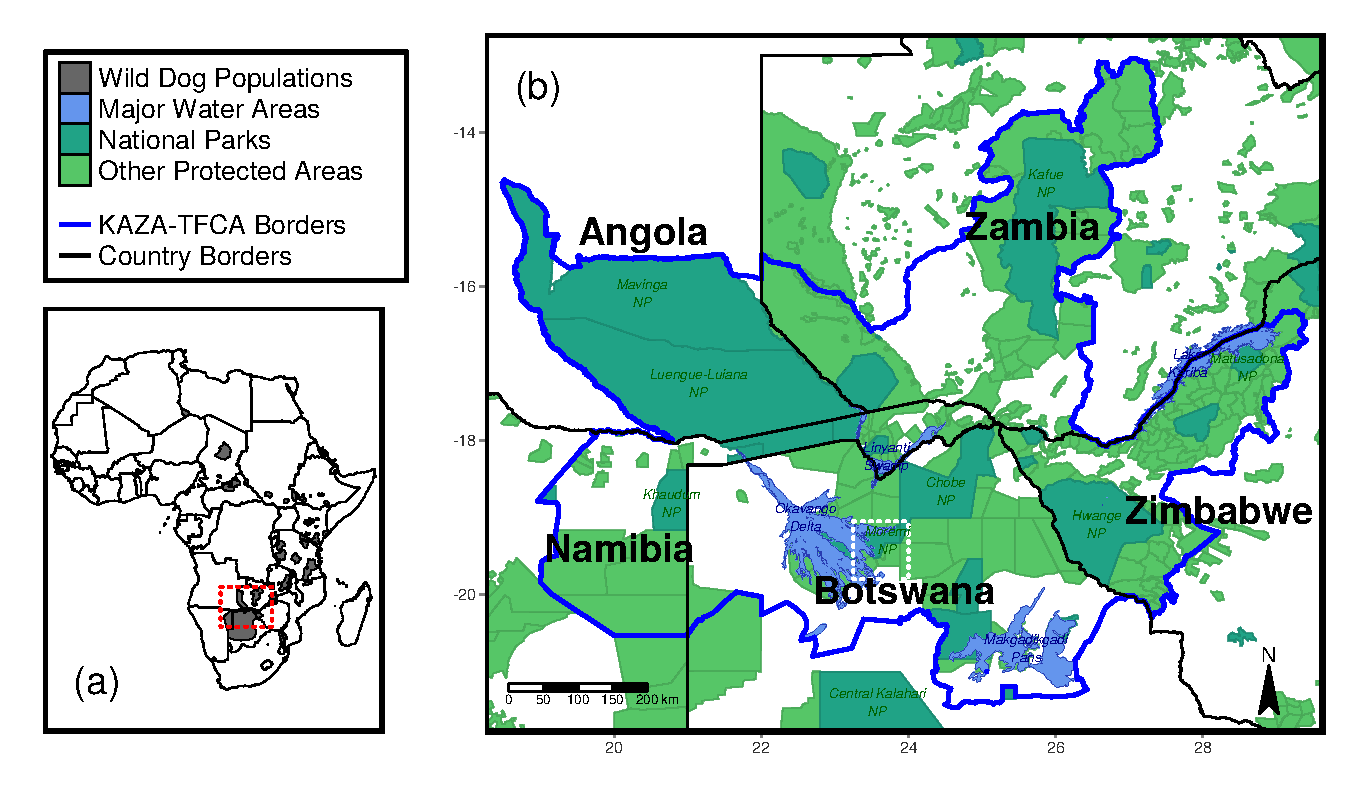
\includegraphics[width = \textwidth]{99_StudyArea.png}
  \caption{(a) Location of the study area in Southern Africa across which we
   simulated dispersing African wild dogs. To mitigate edge effects, our study
   area comprised a buffer zone (red polygon) within which we randomized
   covariate values of the habitat layers. (b) The study area was centered on the
   Okavango Delta and encompassed its immediate surroundings. We initiated
   simulated dispersers at random locations within one of the six source areas
   (orange polygons) that we distributed across the delta. Emigration zones
   (purple polygons) served as checkpoints to identify if and where simulated
   dispersers left the close surroundings of the Okavango delta. These zones were
   generated using a set of cutlines (black dotted lines) originating from the
   center of the delta that dissected an elliptical buffer surrounding the delta
   into sections of equal size and in accordance with the cardinal directions.}
  \label{StudyArea}
 \end{center}
\end{figure}

\subsection{Spatial Habitat Layers}
We represented the physical landscape through which dispersers could move by a
set of spatially referenced habitat layers, each with a resolution of 250 m. The
set of layers included water-cover, distance-to-water, tree-cover,
shrub/grassland-cover, and a human influence layer depicting anthropogenic
influences through villages, roads, and agriculture. A detailed description of
the different habitat layers is provided in \citep{Hofmann.2021}. Importantly,
the water-cover and derived distance-to water layers were generated using MODIS
Terra MCD43A4 satellite imagery that was classified into binary water-cover maps
using a ``floodmapping'' algorithm developed by \citep{Wolski.2017}. This
allowed us to generate almost weekly updated ``floodmaps'', thus providing
detailed information about the flood-extent at any given point in time. In
total, we generated 700 floodmaps between the years 2000 and 2019, based on
which we generated a minimal and maximum flood scenario. To create the minimum
(maximum) flood scenario, we averaged the 100 floodmaps with the smallest
(highest) flood extent and generated a binary layer by masking all pixels that
were inundated in less than 50\% of the maps. The resulting maps are presented
in \Cref{FloodExtent}. Ultimately, we combined the habitat layers into two
stacks, one representing the minimum flood scenario, one representing the
maximum flood scenario. To mitigate edge effects during the dispersal
simulation, we followed \cite{Koen.2010} and expanded the spatial extent of the
stacked layers by 20\% and randomized habitat values within the so created
buffer zone (red rectangle in \Cref{StudyArea}a).

\begin{figure}
 \begin{center}
  \includegraphics[width = \textwidth]{99_FloodExtent.png}
  \caption{Flood extent in the minimum (a) and maximum (b) flood scenarios. In
   the minimum flood scenario (a), water stretched across 3'558
   km\textsuperscript{2}, whereas during maximum flood (b) it covered 9'397
   km\textsuperscript{2}. The two maps were generated using 700 remote sensed
   MODIS MCD43A4 satellite images spanning the years 2000 to 2019.}
  \label{FloodExtent}
 \end{center}
\end{figure}

\subsection{Source Areas and Emigration Zones}
We simulated dispersing AWDs originating from six distinct source areas located
in the vicinity of the OD (\Cref{StudyArea}). We placed source areas in regions
that remained dry during both the minimum and maximum flooding scenario and are
known to host viable wild living wild dog populations. While source areas one to
five were located across the delta's periphery, source area six laid in the OD's
center. The selection of distinct source areas served to facilitate the
identification and quantification of the number of successful dispersal events
between different regions of the OD. Besides source areas, we also generated
``emigration zones'' that we used as checkpoints to determine if and where
simulated individuals left the delta's immediate surroundings
(\Cref{StudyArea}). We generated these zones by first overlaying the OD with an
elliptic that we dissected into roughly equally sized polygons in accordance
with cardinal points (\Cref{StudyArea}).

\subsection{Dispersal Simulation}
We used a previously parameterized and validated dispersal model to simulate
dispersal of AWDs. The dispersal model was trained using GPS data of 16 wild dog
coalitions dispersing across northern Botswana \citep{Hofmann.2023} which was
fed into an integrated step-selection function (iSSF, \citealp{Avgar.2016}). In
iSSFs, consecutive GPS locations are converted into steps (the straight-line
traveled between two GPS recordings \citep{Turchin.1998a}) and compared to a set
of \textit{random} steps in a conditional logistic regression framework
\citep{Fortin.2005, Thurfjell.2014, Muff.2020, Fieberg.2021}. Because iSSFs
capitalize on the autocorrelated nature of the collected data, they provide
better estimates of connectivity than traditional resource selection approaches
\citep{Zeller.2016}. The model presented in \cite{Hofmann.2023} comprised of a
movement kernel, describing how dispersers move across the landscape in the
absence of habitat selection, a habitat kernel, indicating preferred or avoided
habitat features, and interactions among the two, i.e. how movement behavior
changes depending on habitat conditions. According to this model, the main
characteristics of AWD dispersal movements are avoidance of water, avoidance of
areas influenced by humans, and a preference for directional and fast movements.
The model parameters are provided in Appendix SX and explained in
\citealp{Hofmann.2023}.

Originating from each of the six source areas, we simulated 2'000 individuals
dispersing for a total of 2'000 steps. 1'000 individuals were simulated assuming
a minimum flood, the remaining 1'000 assuming a maximum flood. This resulted in
the simulation of a total of 12'000 individuals. The simulation procedure was
based on the algorithm described in \cite{Hofmann.2023} and works as follows. A
random location within the source area is defined as starting point. Originating
from the starting point, a set of 25 random steps is generated by sampling step
lengths from a gamma distribution fitted to observed steps (shape = 0.37, scale
= 6'316) and turning angles from a uniform distribution ($-\pi, +\pi$). Along
each random step the underlying spatial covariates are extracted, and relevant
movement metrics are computed. \(\beta-\)estimates from the fitted model are
used to predict the probability of each step for being chosen, given the steps
associated covariates. Among the 25 proposed steps, one is chosen at random
based on assigned probabilities. The location of the animal is updated, and the
procedure is repeated until the desired number of steps is realized. Here, we
simulated each individual for 2'000 steps, corresponding to a dispersal duration
of 400 days and the longest dispersal duration recorded in this study area
\citep{Cozzi.2020, Hofmann.2021}. The simulated trajectories can be understood
as correlated random walks.

\subsection{Derived Metrics}
Based on simulated dispersal trajectories we quantified connectivity and
identified areas of elevated potential for human wildlife conflict. Our
assessment of connectivity was based on the three complementary connectivity
metrics for IBMMs discussed in \cite{Hofmann.2023}. The set of metrics comprised
of \textit{heatmaps}, depicting areas of intense use, \textit{betweenness maps},
highlighting dispersal corridors and bottlenecks and \textit{maps of inter-patch
 connectivity}, visualizing dispersal success, and duration into distinct habitat
patches. We generated heatmaps by superimposing the study area with a grid with
a spatial resolution of 1 km and quantifying the frequency of simulated
trajectories traversing each grid cell. To compute spatially mapped betweenness
scores, we overlaid the study area with a grid that had a resolution of 2.5 km
and determined the frequency at which simulated individuals transitioned from
one grid-cell to another. A cell-transition was said to occur whenever a
simulated step crossed from one grid-cell across or into another. In case the
same individual repeatedly realized the same cell-transition, we only counted a
single transition to avoid emphasis on regions where individuals moved in
circles. This resulted in a weighted edge-list that we used to compute weighted
betweenness scores for each grid-cell, i.e. the importance of the respective
grid-cell in facilitating movement into adjacent areas
\citep{Bastille-Rousseau.2018, Bastille-Rousseau.2021}. Betweenness was computed
using the \textsf{igraph} R-package \citep{Csardi.2006}. Because the
computations associated with calculating betweenness scores are computationally
more demanding, we deemed the grid size of 2.5 km a sensible compromise between
efficiency and resolution. As a final connectivity metric, we computed the
number of successful dispersal events between each of the six distinct source
areas. We coin this type of connectivity ``inter-patch connectivity''. Dispersal
between two areas was said to be successful whenever the trajectory of an
individual leaving one area intersected with the polygon of another area. We
also estimated the number of individuals that left the OD's vicinity and moved
into an emigration zone. To quantify the dispersal durations required to move
between source areas or into emigration zones, we recorded the minimum number of
steps that individuals moved before arriving at the respective destination.
Besides connectivity, we also identified zones with a high potential for human
wildlife conflict. For this, we isolated all simulated locations where simulated
individuals moved within 500 meters of the nearest human-influenced grid-cell.
Based on the so isolated coordinates we generated density maps. To highlight
differences between derived metrics during maximum and minimum flooding, we
computed difference maps for the heatmap, betweenness map, and human wildlife
conflict maps.

\section{Results}
Figures depicting the derived connectivity and human-wildlife conflict maps are
provided in \Cref{Metrics}. Difference maps to visualize the differences between
minimum and maximum flood are given in \Cref{Difference}. For brevity, we will
here focus on system-wide connectivity patterns and only selectively point to
regional results. Local connectivity maps derived for each source-area
separately are presented in the Appendix. As the heatmaps in \Cref{Metrics}a
reveal, the OD acts as major dispersal barrier during maximum flood yet reveals
vital dispersal habitat during minimum flood. Differences between maximum and
minimum flood (\Cref{Difference}a) are particularly pronounced for the region
between source areas 1 and 2, where few dispersers occur during times of maximum
flood. In fact, because the floodwaters of the OD reach almost into Maun, the OD
creates a line of separation between its eastern and western sections. The
separation is further amplified as the city of Maun is avoided by dispersers in
both scenarios. Similar patterns are observed on the betweenness maps
(\Cref{Metrics}b), where several pinch-points and bottlenecks linking source
area 6 to the surrounding source areas exist during minimum flood. During
maximum flood, however, these links vanish and instead a single corridor at the
south-eastern tip of the OD emerges (\Cref{Difference}b). Despite its apparent
importance in linking the eastern and western sections of the delta, it is
evident from (\Cref{Metrics}a) that this corridor is only rarely used,
especially during the maximum flood scenario. As for the potential for human
wildlife conflict, two clusters emerge (\Cref{Metrics}c). The first cluster lies
at the inflow of the Okavango Delta between source areas 4 and 5 and is most
pronounced during minimum flood (\Cref{Difference}c). Another, albeit visually
less distinct, cluster covers the area at the distal end of the OD, stretching
from lake Ngami to Maun. This area appears particularly relevant at maximum
flood (\Cref{Difference}c). Our analysis of inter-patch connectivity further
demonstrates notable differences in dispersal prospects and dispersal durations
depending on the extent of the flood (\Cref{Metrics}d and \Cref{IPCTable}).
While 4139\pm35.95
 simulated dispersers reach
another source area during minimum extent, only
3'627$ \pm $39.09
 do so during maximum extent, thus
indicating an overall decrease in dispersal success of
\input{99_NumberReachingOthersPercentage.tex}\% during maximum flood.
Concomitantly, the average minimum dispersal durations increases by
\input{99_StepsToReachingOthersPercentage.tex}\%, i.e. from
613\pm7.40
 steps to
718\pm8.53
 steps during maximum flood. These
differences are particularly pronounced for individuals dispersing into source
area 6 on Chief's Island. While the area is reached by
1325\pm31.80
 simulated individuals during minimum
flood, only 298\pm17.10
, i.e.
\input{99_NumberReachingArea6Percentage.tex}\% less, arrive there during maximum
flood. Furthermore, the dispersal duration into source area six from any other
source area increases by \input{99_StepsToReachingArea6Percentage}\% from
773\pm15.06
 steps to
919\pm30.18
 steps. In few occasions,
connectivity between some areas increased during maximum flooding, for instance.
Temporary emigration increased from 5'458$ \pm $21.68

to 5'551$ \pm $20.06
 trajectories (i.e.
by \input{99_TemporaryEmigrationPercentage.tex}\%). Permanent emigration increased
from 4'202$ \pm $35.79
 to
4'405$ \pm $35.74
 trajectories (i.e.
by \input{99_PermanentEmigrationPercentage.tex}\%).

\begin{table}
 \caption{(a) Dispersal frequency and (b) duration (in steps) between source
  areas (labeled 1 to 6) and emigration zones (labeled 7 to 14) during minimum
  and maximum flood.}
 \label{IPCTable}
 \includegraphics[width = \textwidth]{99_IPCTable.png}
\end{table}

\begin{figure}
 \begin{center}
  \includegraphics[width = \textwidth]{99_ImmigrationEmigration.png}
  \caption{Number of individuals emigrating from, or immigrating into a specific
  source area (focal area). Colors indicate into which other areas emigrants
  moved or from which other areas immigrants originate. For instance, the most
  left plot in the upper panel shows the number of individuals moving from
  source area 1 into the six other source areas during minimum and maximum
  flood, respectively.}
  \label{EmigrationImmigration}
 \end{center}
\end{figure}

\begin{figure}
  \begin{center}
  \includegraphics[width = \textwidth]{99_Emigration.png}
  \caption{Absolute number of simulated trajectories running into each of the
  designated emigration zones (purple) during minimum and maximum flood.
  Subfigure (a) depicts the total number of emigrating trajectories, including
  temporary emigrants that eventually returned into the OD's vicinity. Subfigure
  (b) only depicts permanent emigration events.}
  \label{Emigration}
  \end{center}
\end{figure}

\begin{figure}
 \begin{center}
  \includegraphics[width = 0.8\textwidth]{99_Metrics.png}
  \caption{(a) Heatmaps, (b) betweenness maps, (c) maps of human wildlife
   conflict, and (d) maps of inter-patch connectivity, derived from simulated
   dispersal events. Left panels were derived from the minimum flood scenario,
   right panels from the maximum flood scenario. Source areas from which
   dispersers were released are numbered 1-6.  The color scale for betweenness
   scores in (b) was square-rooted to improve visibility of corridors with lower
   values. Note that for clarity in (d) we only present links between adjacent
   source areas. Additional, source-specific maps for each of the four metrics
   are provided in the appendix.)}
  \label{Metrics}
 \end{center}
\end{figure}

\begin{figure}
 \begin{center}
  \includegraphics[width = \textwidth]{99_Difference.png}
  \caption{Difference maps generated from the (a) heatmaps, (b) betweenness
   maps, and (c) maps of human wildlife conflict in \Cref{Metrics}. The maps
   depict the difference between maximum and minimum flood for each metric (i.e.
   $Metric_{flood:max} - Metric_{flood:min}$). Orange regions indicate that the
   respective metric was higher during minimum flood, blue regions that the
   metric was higher during maximum flood.}
  \label{Difference}
 \end{center}
\end{figure}

\section{Discussion}
\subsection{Brief Summary}
In this study, we used a previously parameterized and validated movement model
to simulate dispersal trajectories of AWDs across the OD under two extreme
environmental scenarios: one representing minimal flooding and one representing
maximum flooding. This approach allowed us to investigate connectivity patterns
that emerge under extreme environmental conditions, similar to those projected
under climate change. Predictions of flood conditions across the OD under
climate change remain ambiguous, yet it is generally agreed that climate change
will amplify climatic variability and result in either exacerbated or attenuated
flood events. Our two reference scenarios served to approximate these
conditions. By providing a comprehensive set of connectivity maps for both
scenarios, we highlighted how dispersal routes and prospects of the endangered
AWD changed depending on flood conditions. Our simulations revealed that the
propensity to move between the eastern and western sections of the OD decreased
significantly during maximum flood. This effect likely resulted from the
combined influence of floodwaters and anthropogenic pressures, which together
formed a dispersal barrier that limited connectivity. When flooding was at a
minimum, on the other hand, the retracted floodwaters revealed vital dispersal
habitats that facilitated movement between the western and eastern regions of
the OD. Anecdotal evidence supports the notion that vital dispersal habitats are
only available during periods of low flood, for the only dispersal coalition
recorded to successfully move between the eastern and western delta using GPS
data was observed at a time of minimal flooding  \citep{Cozzi.2020}. The lack of
dispersal habitat during maximum flood also resulted in an almost complete
isolation of Chief's Island, the OD's central peninsular (source area 6 in
\Cref{StudyArea}b). The peninsular itself remains remains dry in both scenarios,
yet becomes entirely surrounded by water during times of maximum flood. This
limits pathways to emigrate or immigrate and results in low dispersal prospects
for individuals moving towards this area. Despite the general reduction of
connectivity and increased dispersal durations during maximum flood, the number
of dispersers moving between some of the source areas increased during maximum
flood. This was, for instance, the case for movements between sour areas 1 and 4
and likely resulted from individuals that were deflected by the expanded flood
and redirected into more accessible habitats. The deflection of individuals by
the flood also had direct implications for the spatial arrangement of dispersal
corridors as movement routes that traverse the central parts of the OD
disappeared and more individuals were funneled through a corridor running
along the southern fringes of the OD.

\subsection{Validating Predictions}
Although the movement model underlying our simulations was validated using
independent dispersal data (see \citealp{Hofmann.2023}), assessing the
reliability of our predictions for the two extreme flooding scenarios remains
challenging. Firstly, because collecting data of dispersing individiauls is
difficult \textit{per se} \citep{Fattebert.2015, Cozzi.2020} and, secondly,
because flood-conditions akin to those studied here only occur rarely
\citep{Wolski.2017}. Dispersers typically only make up for a small proportion of
the entire population and predicting the timing of dispersal is often
non-trivial. Coupled with the limited battery-lifetime of most conventional GPS
collars, it is logistically unfeasible to collected large amounts of GPS data
during dispersal. However, as an alternative to GPS data, genetic or
observational data could also yield insight into functional connectivity.
Genetic data is often viewed as ultimate measure of functional connectivity
\citep{Baguette.2013} and thus often serves as validation of connectivity maps
(e.g. \citealp{Cushman.2010} or \citealp{Spear.2010}). Genetic analysis across
southern Africa revealed moderate levels of dispersal and identified a
genetically particularly diverse population cluster located near northern
Botswana \citep{Tensen.2022}. While such analyses provide valuable insights into
long-term dispersal patterns, they are unlikely to yield insights on short-term
connectivity patterns such as those studied here. Observational data, on the
other hand, readily delivers information on seasonally changing dispersal
patterns. Such data may not only be collected by trained field assistants, but
could also be obtained through photographic evidence from tourists in a
citicen's science approach. AWDs, as well as most other large carnivores, are
individudally identifiable, either by their coat pattern or other unique
features. Given a set of georeferenced images, individuals can thus be traced
through space and time. \cite{Cozzi.2013} provide first evidence on the
usefulness of this approach. As of today, however, the moderate amount of data
collected and spatially biased sampling effort prohibits using such data for
validation purposes. Finally, our representation of the flood was, by design,
focused on rare extreme events. Since the beginning of our dataset.
Consequently, the amount of data suitable for validation is limited.

\subsection{Climate Change in the Okavango Delta}
Despite the importance of the OD as a driver of ecosystem functioning, species
distribution, and dispersal corridors, predicting flood patterns under future
conditions has proven notoriously difficult \citep{Wolski.2008}. This is owed to
the intricate interplay between climatic conditions, anthropogenic water usage,
and the topographic peculiarities of the region. In regard to climatic
conditions, Southern Africa is projected to face temperature rises above the
global average \citep{Engelbrecht.2015}. According to predictions, this will
cause a more intense but shorter rainy season in Botswana \citep{Akinyemi.2019}.
Precipitation across the ODs catchment areas in Angola is expected to increase
but it remains unclear whether elevated precipitation levels will be offset by
increased temperatures and accelerated evapotranspiration \citep{Wolski.2008,
Moses.2018}. In a recent study, \cite{Wolski.2008} used three competing climate
models and predicted that conditions across the delta may range from ``much
wetter'' to ``much drier''. Accurate predictions of future conditions across the
OD are further hindered by multi-decadal oscillations in precipitation patterns
in Angola that cause shifts between wet and dry periods and may offset or
amplify long term trends over short periods \citep{Wolski.2008, Wolski.2012}.
Besides climatic uncertainties, the OD's future is plagued by socio-economic
uncertainties. The OD and its tributaries represent important water-sources for
adjacent communities and are subject to intense developmental debates about
future abstractions. These result from an ever-growing human population,
increasing socio-economic needs, and resettlement in Angola following peace
\citep{Kgathi.2006} and have culminated in large uncertainties regarding the
dimensions of future water abstractions \citep{Hughes.2011}. Although upstream
abstractions along the Okavango River are thought to have relatively little
impact on the flooding pattern of the OD, the combined effects of climate change
and anthropogenic abstractions could result in significant ``delta-drying''
\citep{Murray-Hudson.2006}. A final complicating factor is the OD's shallow
gradient (1:3300, \citealp{Gumbricht.2004}) in result to which water only slowly
descends through the OD. Hippos dredge many of the slow-moving waterways and
thereby ensure a steady flow of water, yet their behavior can also lead to the
creation of new waterways and thus to a spatial redistribution of floodwater
across the delta \citep{McCarthy.1998a}. In summary, the significant
uncertainties regarding future flood conditions preclude clear predictions of
connectivity and complicate the protection and preservation of important
movement corridors, especially in light of climate change. Thus, instead of
anticipating and preparing for a single, clearly defined scenario, conservation
authorities must maintain flexibility and develop a multitude of strategies that
can be applied to each case.

\subsection{Social Resistance}
Here, we focused on the influence of environmental resistance on dispersal but
disregarded the impact of social resistance. That is, while our simulation
rendered how environmental features affect dispersal behavior, it neglected
potential interactions between dispersing AWDs and their conspecifics,
predators, or pray. This was a simplifying assumption and owed to a lack of data
on sympatric species at the appropriate temporal and spatial scale. According to
the social resistance hypothesis, however, dispersers' movement patterns are
likely to be driven not only by environmental features, but by a combination of
environmental-, intra-, and interspecific conditions \citep{Armansin.2019}.
Together, intra- and inter-specific factors are sometimes referred to the
\textit{social landscape} through which dispersers move and are thought to be
important drivers of dispersal behavior \citep{Wey.2015}. Previously, this has
been demonstrated for dispersing meerkats (\textit{Suricata suricatta}), a
species surprisingly similar to the AWD in terms of its social organization and
dispersal behavior \citep{Cozzi.2018}. Similarly, it has been discovered that
AWDs rely on shared marking sites to advocate presence and reproductive status
\citep{Apps.2022, Claase.2022}. Although the sites are primarily used by
resident AWDs, even dispersers or competing species use them occasionally to
obtain information on the presence of local packs. In fact, dispersers may use
the marking sites to more effectively navigate the social landscape and avoid
competitors or locateother-sex dispersal coalitions. Besides such intra-specific
factors, also the distribution and abundance of prey can be expected to have
direct consequences on dispersal routes, as dispersers are usually in search of
suitable, i.e. prey-rich, territory to settle. This goes to show that accounting
for the social landscape will no only add another level of realism, but also
additional complications. Interacting species cannot be considered as
independent of each other, meaning that the impact of climate change on one
species will result in trophic cascades affecting several species at once with
substantial alterations in the community composition \citep{Thuiller.2006}.

AWDs primarily prey on species that are either restricted by access to water or
by the forage growing in its close proximity. Attraction of prey to water is
particularly evident during the dry season, when pans and puddles dry up and
forage becomes scarce across the landscape. During these periods, floodplains
serve as fallback habitat and attract large herds of ungulates that forage near
rivers and streams filled by floodwater \citep{Bonyongo.2005, Bennitt.2014}. We
previously reported that dispersing AWDs also prefer moving near water sources,
likely in an attempt to track their prey \citep{Hofmann.2021}. However, a
reduction in the spatial extent of flood and associated losses in floodplain
habitats could lead to increased concentration of prey and intensified
competition among large carnivores. Within this carnivore community, AWDs are
inferior predators and face challenges in competition with lions, spotted
hyenas. Resident or dispersing AWDs that avoid superior competitors in space or
time may get forced into areas of moderate prey-availability \citep{Droge.2017}.
An increased flood-level, on the other hand, will likely limit the amount of
suitable habitat across the OD's landscape. Recent research on lions has
demonstrated that flooding reduces the carrying capacity of the system for
lions, resulting in a crowing within remaining habitats and increased
competition. It is, however, unclear how an incrased flood level will affect
inter-specific competition and whether AWDs will persist under elevated levels
of intra-guild competition.

\subsection{Anthropogenic Resistance}
To this day, the social acceptance of AWDs among the local population of
northern Botswana has not been investigated. This prohibits a deeper
understanding of the anthropogenic resistance experienced by dispersing
individuals \citep{Ghoddousi.2021}. Talk a bit about anthropogenic resistance.
While our dispersal model rendered dispersers' behavior with regards to the
presence of humans, it did not take human bheavior into account. This is
generally referred to as anthropogenic resistance. The employed dispersal model
rendered how biophysical elements and anthropogenic presence influence dispersal
movements. It did not, however, account for social or anthropogenic resistance.
Corridors that are estimated based on landscape features only may over- or
under-estimate true connectivity. Overestimate in areas where there is strong
anthropogenic resistance (e.g. hunting, trapping) - Underestimate in areas where
humans facilitate movements (e.g. through supplementary food supplies). The
flood might funnel individuals into unsafe areas with high risk of human-caused
mortality \citep{Northrup.2012} (i.e. ecological traps). Depending on the flood,
individuals get funneled towards different regions of high anthropogenic
influence, suggesting that climate change may induce spatial shifts in regions
with a high potential for human wildlife conflict. Depending on the level of
anthropogenic resistance that dispersing wild dogs experience in the different
areas, these regions may act as ecological traps into which individuals get
funneled due to external conditions.

% Comparable observations have been made by \cite{Towns.2009}, who show that
% annual fluctuations in sea-ice extent forces polar bears \textit{Ursus
% maritimus} to move onshore and more proximal to humans, thus increasing the
% likelihood for HWC. Consequently, human wildlife conflict may be viewed not as
% static, but dynamic variable that is prone to seasonal fluctuations and long
% term climatic trends. This is also what \cite{Kitratporn.2022} find. They report
% that human wildlife conflict with elephants is expected to increase in some
% areas (where habitat suitability increases) but to decrease in others (where
% habitat suitability decreases).

% For example, \cite{Michalski.2006} report elevated live-stock depredation by
% \textit{Puma concolor} and \textit{Panthera onca} on cattle ranches in close
% proximity to forest corridors. Similarly, changing water temperatures and
% associated shifts in prey-availability have resulted in white sharks moving in
% closer vicinity to humans ultimately resulting in an increased frequency of
% shark attacks\citep{Chapman.2016}.

\subsection{Human Wildlife Conflict}
It is well documented that a close proximity between humans and wildlife
increases the likelihood of human-wildlife conflict (e.g.
\citealp{Michalski.2006} or \citealp{Chapman.2016}). It can thus be expected
that areas where dispersers move into proximity of human-dominated landscapes
hold an increased potential for human-wildlife-conflict (HWC). It has been
suggested that climate change will increase competition between humans and
wildlife for scarce resources and thereby exacerbate HWC globally
\cite{Abrahms.2021}. Our simulations suggest that dispersers may indeed utilize
different routes depending on flood conditions. In our case, tthis did not
result in an overall increase in HWC, but we observed a regional shift of where
dispersers come into the vicinity of human-dominated areas. During minimum
flood, these areas were most prominent along the OD's panhandle, where the
Okavango River enters the alluvial fan of the OD. The panhandle is inhabited
comparably densely ($\input{99_HumanDensityPanhandle.tex}$ inh. /
km\textsuperscript{2}) and used for both agricultural farming
($\input{99_AgriculturePanhandle.tex}$\% covered by agricultural fields) and
livestock farming ($\input{99_CattleDensityPanhandle.tex}$ cattle /
km\textsuperscript{2}). It has previously received attention as a hotspot for
human-wildlife conflict due to livestock depredation by carnivores
\citep{LeFlore.2019} and repeated elephant raids \citep{Buchholtz.2020}. During
maximum flood, in contrast, a larger number of dispersers moved into proximity
of Maun and the adjacent region of Lake Ngami at the southern fringes of the OD.
Maun is the biggest and most densely populated city in the study area
($\input{99_HumanDensityMaun.tex}$ inh. / km\textsuperscript{2}) and serves as
hub for touristic excursions into the OD. It's surrounding area is
agriculturally less intensively used ($\input{99_AgricultureMaun.tex}$\% covered
by agricultural fields) but the livestock density is comparably high
($\input{99_CattleDensityMaun.tex}$ cattle / km\textsuperscript{2}). Despite
this and the fact less than 3\% of livestock depredations can be linked to AWDs,
there have been numerous occasions where AWDs were harmed or killed within the
city's proximity \citep{Gusset.2009, Cozzi.2020}. While the panhandle and the
city of Maun themselves are unprotected, they are located near formally
protected areas and may thus serve as ecological traps for wildlife leaving the
surrounding protected areas \citep{Woodroffe.1998, Northrup.2012}. Dispersing
individuals appear to be particularly at risk, as they readily venture outside
protected areas into hostile landscapes \citep{Elliot.2014, Cozzi.2020}. In
Zambia, dispersal and the associated mortality have caused deterioration of
genetic diversity and resulted in the ned loss of individuals
\citep{Leigh.2012}. Recent genetic analyses across southern Africa, in contrast,
identified a genetically diverse population cluster near northern Botswana,
suggesting moderate levels of dispersal \citep{Tensen.2022}. Nevertheless,
anticipating how climate change and the associated changes in the biophysical
landscape through which dispersers move will impact hWC will be paramount to
prioritize efforts and more efficiently conserve and sustain dispersal pathways.

\subsection{Conclusion}
Our dispersal simulations across two extreme environmental scenarios revealed
striking differences in dispersal prospects and landscape connectivity for
dispersing AWDs. We thereby showed that extreme environmental conditions, akin
to those projected under climate change, will have important impacts on
functional connectivity and may alter areas of HWC. Given the complexity of the
studied ecosystem and its associated intricate feedback loops, predictions of
future conditions remain challenging and plagued by uncertainty. Wildlife
managers and conservation bodies therefore need to move beyond focusing on
single scenarios and consider multiple possibilities to adequately respond to
changes in the environment due to climate change, while also coping with the
socio-economic needs of an ever-expanding human population. This will require
the development of protection strategies that can accommodate both more extreme
pronounced, or less intense flood. Successful conservation strategies will be of
particular relevance for wide-ranging, endangered species that are already at
the verge of extinction, such as the African wild dog.

\section{Authors' Contributions}
D.D.H., G.C., D.M.B., A.O. and conceived the study and designed methodology;
D.D.H., G.C., D.M.B., and J.W.M. collected the data; D.D.H. analysed the data;
G.C., D.M.B., and A.O. assisted with modeling; D.D.H., G.C., and D.M.B.wrote the
first draft of the manuscript and all authors contributed to the drafts at
several stages and gave final approval for publication.

\section{Data Availability}
Access to R-scripts to replicate our anlaysis will be provided through an online
repository at the time of publication.

\section{Acknowledgements}
We thank the Ministry of Environment and Tourism of Botswana for granting
permission to conduct this research. We thank C. Botes, I. Clavadetscher, and G.
Camenisch for assisting with wild dog immobilizations. We also thank B. Abrahms
for sharing her data of three dispersing wild dogs. This study was funded by
Albert-Heim Foundation, Basler Stiftung für Biologische Forschung, Claraz
Foundation, Idea Wild, Jacot Foundation, National Geographic Society, Parrotia
Stiftung, Stiftung Temperatio, Wilderness Wildlife Trust Foundation,
Forschungkredit der Universität Zürich, and a Swiss National Science Foundation
Grant (31003A\_182286) to A. Ozgul.

\newpage
\begingroup
\singlespacing
\bibliography{Literature}
\endgroup

\end{document}
